\documentclass[conference]{IEEEtran}
\IEEEoverridecommandlockouts

\usepackage{amsmath,amssymb,amsfonts}
\usepackage{algorithmic}
\usepackage{graphicx}
\usepackage{textcomp}
\usepackage{xcolor}
\usepackage{booktabs}
\usepackage{microtype}
\usepackage{cite}
\usepackage{url}

\graphicspath{{../figures/}{figures/}}
\urldef{\repolink}\url{https://github.com/Rhriti/sequential-boxing-judging}

\begin{document}

\title{Sequential Prediction of Professional Boxing Round Outcomes: Evaluating Scorecard State and Recurrent Memory Beyond Punch Statistics\thanks{Code and result tables: \repolink.}}

\author{\IEEEauthorblockN{Hritij Rana}
\IEEEauthorblockA{\textit{Department of Computer Science and Engineering} \\
\textit{Netaji Subhas University of Technology} \\
Delhi, India \\
hritij.rana.pg26@nsut.ac.in}}

\maketitle

\begin{abstract}
Under the regulatory 10-Point Must System in professional boxing, ringside judges are instructed to evaluate each three-minute round as an independent athletic contest. However, human decision-makers frequently exhibit sequential biases, such as compensatory officiating and score balancing. In this work, we investigate whether running scorecard state provides predictive signal for round winners beyond high-dimensional punch statistics, and whether deep sequence models can exploit this history. Analyzing 13,776 judge-round evaluations across 2,061 bout-judge timelines from the Jabbr DeepStrike dataset, we estimate fixed-effects econometric models alongside supervised machine learning algorithms. We provide rigorous evidence of compensatory ``catch-up'' bias: trailing fighters on a judge's card enjoy a statistically significant scoring advantage ($\beta = -0.3016$, $p = 1.40 \times 10^{-36}$), supporting Hypothesis 1. However, contrary to the hypothesis that sequential bias intensifies under late-bout pressure ($H_2$), we find that catch-up behavior significantly attenuates in championship rounds 11--12 ($\beta = +0.0990$, $p = 1.18 \times 10^{-4}$). In supervised out-of-sample evaluation across five bout-grouped folds, gradient boosted decision trees (XGBoost) achieve a held-out log loss of 0.468 (accuracy 76.7\%), whereas a causal Cognitive Bias Sequence Network (CBSN) with gated LSTM memory yields a log loss of 0.483 (accuracy 76.1\%). Dynamic attention weights demonstrate that judge dependence on bout history decays from 0.418 in early rounds to 0.307 in late rounds. While causal memory ablation confirms that recurrent history boosts trailing-corner win probability by 0.073, the added parametric complexity of neural sequence models fails to surpass tree baselines on short, noisy athletic sequences.
\end{abstract}

\begin{IEEEkeywords}
Combat sports analytics, sequential decision-making, compensatory bias, sports officiating, recurrent neural networks, gradient boosting, 10-Point Must system.
\end{IEEEkeywords}

\section{Introduction}
Professional boxing officiating is governed by the 10-Point Must System, codified by regulatory bodies such as the Association of Boxing Commissions (ABC) and the World Boxing Council (WBC)~\cite{abc2017,wbc2020}. Under statutory guidelines, three ringside judges score each round independently on a 10--9 scale (barring knockdowns or point deductions) based on clean punching, effective aggressiveness, ring generalship, and defense. A foundational assumption of this regulatory design is round independence: the scoring of round $r$ must depend strictly upon the athletic events occurring within round $r$, invariant to rounds $1, \dots, r-1$.

Despite formal mandates, human arbiters across professional sports exhibit documented sequential dependencies~\cite{garicano2005,dohmen2008,chen2016}. Umpires in Major League Baseball, referees in European football, and judges in Olympic combat sports frequently engage in compensatory decision-making---subconsciously penalizing leading competitors or awarding marginal exchanges to trailing competitors to maintain apparent parity or correct perceived past errors~\cite{peters2014,myers2006,moskowitz2012}. In professional boxing, where scorecards are kept confidential until the conclusion of the contest, judges retain internal psychological tallies of their own scorecards, introducing the potential for cognitive anchoring and sequential evaluation bias.

While previous machine learning approaches to combat sports have focused primarily on computer-vision punch detection and static round-by-round scoring~\cite{duboef2021,jabbr2023}, they treat rounds as exchangeable, identically distributed observations. Static models neglect the sequential state of the bout. 

In this paper, we formulate round-outcome prediction as a sequential supervised learning task: predicting whether judge $j$ awards round $r$ to the red-corner fighter given objective computer-vision punch metrics, the judge's prior scorecard margin, and recurrent bout history. We evaluate models using binary log loss as the primary metric and classification accuracy as secondary, under a strict 5-fold bout-grouped cross-validation design that prevents information leakage across rounds or judges of the same contest.

The key contributions of this paper are fourfold:
\begin{enumerate}
    \item \textbf{Econometric Proof of Compensatory Judging:} Using a fixed-effects logistic regression framework ($N = 13,776$) with bout and judge fixed effects and cluster-robust standard errors, we establish that judges display strong compensatory catch-up behavior ($H_1$: $\beta = -0.3016$, $p < 10^{-35}$).
    \item \textbf{Refutation of Late-Round Intensification:} We test whether catch-up bias escalates during championship rounds 11--12 ($H_2$). Surprisingly, the empirical interaction is positive ($\beta = +0.0990$, $p = 1.18 \times 10^{-4}$), proving that compensatory bias attenuates as bout finality approaches.
    \item \textbf{Causal Recurrent Sequence Architecture:} We develop the Cognitive Bias Sequence Network (CBSN), a causal gated recurrent architecture with judge embeddings and an objective skip connection, guaranteeing zero temporal leakage. Dynamic attention weights illustrate a steady decline in historical memory reliance from $0.418$ in early rounds to $0.307$ in late rounds.
    \item \textbf{Empirical Limits of Deep Sequence Models:} Through rigorous held-out cross-validation, we demonstrate that while sequential features improve over static models, XGBoost outperforms the causal LSTM (log loss 0.468 vs.\ 0.483; accuracy 76.7\% vs.\ 76.1\%), highlighting the inductive advantages of tree-based models on compact, noisy athletic sequences.
\end{enumerate}

\section{Related Work}
\subsection{Combat Sports Analytics and Punch Tracking}
Quantitative analysis in boxing historically relied on manual punch counts (e.g., CompuBox), which suffer from observer fatigue and subjective classification errors. Recent advances in computer vision, particularly the DeepStrike tracking system developed by Jabbr AI~\cite{jabbr2023}, extract 30+ standardized biomechanical and tactical variables per round, including punch velocity, connection quality, impact, defensive head movement, and spatial dominance. duBoef et al.~\cite{duboef2021} developed an objective punch-stat model using regularized $L_1$ logistic regression to predict consensus round outcomes. While their model demonstrated high alignment with official scores, it operated purely in a static regime, ignoring the sequential state of the contest.

\subsection{Sequential Bias and Compensatory Officiating}
A rich literature in behavioral economics demonstrates that human arbiters are prone to sequential distortion. Chen, Moskowitz, and Shue~\cite{chen2016} documented decision-making under the gambler's fallacy among asylum judges, loan officers, and baseball umpires, finding that arbiters actively avoid making consecutive identical calls. In professional soccer, Garicano et al.~\cite{garicano2005} and Dohmen~\cite{dohmen2008} revealed referee favoritism and injury time distortions driven by social pressure. Peters and van Ours~\cite{peters2014} formalized compensatory refereeing, showing that referees award questionable penalties to balance prior controversial decisions. In boxing, Balmaceda et al.~\cite{balmaceda2014} analyzed middlemost scoring aggregation to mitigate outlier judges, but empirical research quantifying within-judge sequential scorecard adjustments has remained limited.

\section{Data and Prediction Task}
\subsection{The Jabbr DeepStrike Dataset}
We analyze the paired DeepStrike dataset from Jabbr AI~\cite{jabbr2023}, comprising professional boxing matches recorded with multi-camera computer-vision tracking paired with official ringside scorecards. Each bout includes synchronized round-level punch and positional features for both the red and blue corners, alongside official scorecard entries from three ringside judges. 

Following standard regulatory convention, we restrict analysis to standard 10--9 rounds (which constitute over 96\% of all completed professional rounds) occurring in rounds $r \ge 2$, where sequential scorecard history exists. The resulting balanced panel contains $N = 13,776$ judge-round evaluations across 2,061 judge-bout timelines from 687 distinct professional bouts.

\subsection{Punch Feature Space}
For each round $r$ of bout $i$, the computer vision pipeline extracts 30 differential features capturing relative performance between the red and blue corners ($x_{ir} \in \mathbb{R}^{30}$). These features encompass:
\begin{itemize}
    \item \textit{Volume and Efficiency:} Accuracy differential, landed punch share, thrown punch share, total landed, total thrown.
    \item \textit{Impact and Commitment:} High-impact power punches, maximum force punches, low- and high-commitment missed punches.
    \item \textit{Punch Typology:} Differentials in single punches, lead punches, rear hands, head shots, body shots, straights, hooks, overhands, and uppercuts.
    \item \textit{Ring Generalship and Stance:} Spatial distance pressure, movement pressure, positional ring center dominance, combination aggression, power aggression, and stance differentials (orthodox, southpaw, squared).
\end{itemize}

\subsection{Formal Task Formulation and Non-Leakage Guarantees}
Let $y_{ijr} \in \{0, 1\}$ denote the binary outcome indicating whether judge $j$ in bout $i$ awarded round $r$ to the red corner ($y_{ijr} = 1$) or the blue corner ($y_{ijr} = 0$).

To evaluate sequential cognitive bias without temporal leakage, we define the running scorecard margin strictly prior to round $r$:
\begin{equation}
\Delta_{ij,r-1} = \sum_{t=1}^{r-1} \left( s_{ijt}^{\text{red}} - s_{ijt}^{\text{blue}} \right),
\end{equation}
where $s_{ijt}^{\text{red}}, s_{ijt}^{\text{blue}} \in \{9, 10\}$ represent the official points awarded by judge $j$ in round $t$. A positive margin $\Delta_{ij,r-1} > 0$ indicates that the red fighter leads on judge $j$'s card entering round $r$, whereas $\Delta_{ij,r-1} < 0$ indicates a blue lead.

We also construct a late-round indicator $L_r = \mathbb{I}(r \ge 11)$ identifying championship rounds (rounds 11 and 12), and its interaction term:
\begin{equation}
\text{LateInteraction}_{ijr} = \Delta_{ij,r-1} \times L_r.
\end{equation}
Crucially, all sequential signals available to predict round $r$ are strictly causal: punch features reflect only round $r$, and scorecard variables reflect only rounds $1, \dots, r-1$.

\section{Methodology and Predictive Models}

\subsection{Stage 1: Objective Punch Baseline ($\hat{P}$)}
To isolate the influence of objective round action from subjective bias, we reproduce the duBoef et al.~\cite{duboef2021} benchmark. We fit an $L_1$-regularized logistic regression on the 30 standardized DeepStrike differential features:
\begin{equation}
\hat{P}_{ir} = \sigma\left( \mathbf{w}^{\top} x_{ir} + b \right),
\end{equation}
where $\sigma(z) = (1 + e^{-z})^{-1}$. The fitted scalar $\hat{P}_{ir} \in (0, 1)$ represents the objective probability that a round belongs to the red corner based solely on punch statistics. In 5-fold cross-validation, Stage 1 achieves a held-out classification accuracy of 73.8\%.

\subsection{Stage 2A: Fixed-Effects Econometric Models}
To test behavioral hypotheses regarding sequential bias, we estimate nested logistic regressions with judge fixed effects $\gamma_j$ and bout fixed effects $\alpha_i$, with standard errors clustered at the bout level:
\begin{itemize}
    \item \textbf{Model $M_0$ (Objective Baseline):}
    \begin{equation}
    \text{logit}(P(y_{ijr}=1)) = \beta_1 \hat{P}_{ir} + \alpha_i + \gamma_j.
    \end{equation}
    \item \textbf{Model $M_1$ (Sequential Catch-Up):}
    \begin{equation}
    \text{logit}(P(y_{ijr}=1)) = \beta_1 \hat{P}_{ir} + \beta_2 \Delta_{ij,r-1} + \alpha_i + \gamma_j.
    \end{equation}
    \item \textbf{Model $M_2$ (Full Econometric Specification):}
    \begin{align}
    \text{logit}(P(y_{ijr}=1)) = &\;\beta_1 \hat{P}_{ir} + \beta_2 \Delta_{ij,r-1} \nonumber \\
    &+ \beta_3 (\Delta_{ij,r-1} \times L_r) + \alpha_i + \gamma_j.
    \label{eq:m2}
    \end{align}
\end{itemize}
Under Hypothesis 1 ($H_1$: compensatory catch-up), $\beta_2 < 0$: a leading fighter entering round $r$ faces a reduced log-odds of winning round $r$. Under Hypothesis 2 ($H_2$: championship escalation), $\beta_3 < 0$: the compensatory pressure magnifies in rounds 11--12. 

\textit{In-Sample Note:} Model $M_2$ achieves an in-sample accuracy of 83.3\%. However, because bout fixed effects $\alpha_i$ are unobservable for a newly encountered bout, $M_2$ serves as an explanatory econometric model rather than an out-of-sample predictor.

\subsection{Stage 2B: Gradient Boosted Trees (XGBoost)}
For out-of-sample supervised evaluation, we train an XGBoost classifier~\cite{chen2016xgboost} using 32 features: the 30 raw DeepStrike punch metrics, the lagged card margin $\Delta_{ij,r-1}$, and the late round indicator $L_r$. We exclude $\hat{P}$ to avoid circular leakage from Stage 1 full-sample estimation. Hyperparameters (learning rate 0.05, max depth 4, subsample 0.8, early stopping on inner validation) are tuned exclusively on training folds.

\subsection{Stage 3: Cognitive Bias Sequence Network (CBSN)}
To capture potential non-linear temporal dependencies across rounds, we design the CBSN architecture. For each bout-judge timeline, rounds are processed causally from round 1 through $R$. 

When evaluating round $r$, the network maintains an LSTM cell~\cite{hochreiter1997} with 16 hidden units whose hidden state $h_{r-1}$ incorporates rounds $1, \dots, r-1$. The network computes:
\begin{align}
h_{r-1} &= \text{LSTM}(x_1, \dots, x_{r-1}), \\
e_j &= \text{Embedding}(j; d=4), \\
w_{\text{hist}} &= \sigma\left( W_a [x_r; h_{r-1}; e_j] + b_a \right), \\
w_{\text{imm}} &= 1 - w_{\text{hist}}, \\
z_{\text{gated}} &= w_{\text{imm}} \cdot f_{\text{imm}}(x_r) + w_{\text{hist}} \cdot f_{\text{hist}}(h_{r-1}), \\
\hat{y}_{ijr} &= \sigma\left( z_{\text{gated}} + W_{\text{skip}} x_r + b_0 \right),
\end{align}
where $e_j \in \mathbb{R}^4$ is a learned judge embedding, and $W_{\text{skip}}$ provides an objective skip connection directly from current round punch stats $x_r$ to the output logit. The model contains $k = 3,214$ trainable parameters and is trained with Adam ($10^{-3}$, weight decay $10^{-4}$, dropout 0.3) for 80 epochs.

\begin{figure}[t]
\centering
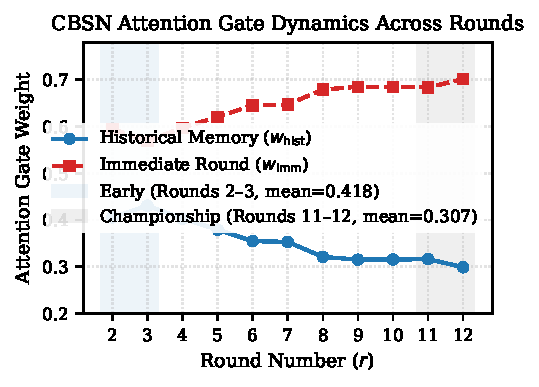
\includegraphics[width=0.92\columnwidth]{fig1_attention_by_round.pdf}
\caption{Dynamic attention gate weights in the Cognitive Bias Sequence Network (CBSN) across rounds 2 through 12. Reliance on historical memory ($w_{\text{hist}}$) peaks in round 3 (0.431) and systematically decays to 0.299 in round 12, while immediate round punch weight ($w_{\text{imm}}$) rises to 0.701.}
\label{fig:attention}
\end{figure}

\section{Experimental Setup}
\subsection{Cross-Validation Protocol}
All predictive evaluations employ 5-fold bout-grouped cross-validation (`GroupKFold`). Because rounds and judges within a bout share unobserved bout-specific dynamics, all rounds and all three judges for any given bout are assigned strictly to either the training set or the test set. The exact same fold assignments (verified by SHA-1 checksums) are shared across XGBoost and CBSN.

\subsection{Evaluation Metrics}
Following best practices for probabilistic scoring models, the \textbf{primary metric} is held-out binary log loss (cross-entropy):
\begin{equation}
\mathcal{L} = -\frac{1}{N_{\text{test}}} \sum_{m=1}^{N_{\text{test}}} \left[ y_m \log \hat{p}_m + (1 - y_m) \log (1 - \hat{p}_m) \right].
\end{equation}
Classification accuracy (threshold at 0.5) is reported as a secondary metric. For nested econometric models, we report log-likelihood ($\text{LLF}$), Akaike Information Criterion ($\text{AIC}$), Bayesian Information Criterion ($\text{BIC}$), and likelihood-ratio ($\text{LR}$) test statistics.

\section{Empirical Results}

\subsection{Econometric Evaluation of Sequential Bias (Table I)}
Table~\ref{tab:econometrics} summarizes the estimation results for Models $M_0$, $M_1$, and $M_2$ on the full panel of 13,776 judge-rounds. 

\begin{table}[t]
\caption{Econometric Fixed-Effects Logistic Regression Results}
\label{tab:econometrics}
\centering
\footnotesize
\setlength{\tabcolsep}{3.5pt}
\begin{tabular}{lccc}
\toprule
\textbf{Variable / Metric} & \textbf{Model $M_0$} & \textbf{Model $M_1$} & \textbf{Model $M_2$} \\
\midrule
$\hat{P}_{ir}$ (Punch Baseline) & 6.955*** & 7.010*** & 7.055*** \\
 & (0.288) & (0.290) & (0.294) \\
$\Delta_{ij,r-1}$ (Card Margin) & --- & -0.269*** & -0.302*** \\
 & & (0.023) & (0.024) \\
$\Delta \times \text{Late}$ (Championship) & --- & --- & 0.099*** \\
 & & & (0.026) \\
\midrule
Judge Fixed Effects & Yes & Yes & Yes \\
Bout Fixed Effects & Yes & Yes & Yes \\
Observations ($N$) & 13,776 & 13,776 & 13,776 \\
Log-Likelihood ($\text{LLF}$) & -4991.78 & -4828.87 & -4817.02 \\
AIC & 12,191.55 & 11,867.74 & 11,846.03 \\
BIC & 20,505.43 & 20,189.14 & 20,174.97 \\
In-Sample Accuracy & 82.3\% & 83.1\% & 83.3\% \\
\midrule
LR Test vs.\ $M_0$ ($\chi^2$) & --- & 325.82*** & 349.52*** \\
LR Test vs.\ $M_1$ ($\chi^2$) & --- & --- & 23.71*** \\
\bottomrule
\multicolumn{4}{l}{\scriptsize Standard errors clustered by bout in parentheses. *** $p < 0.001$.}
\end{tabular}
\end{table}

\textbf{Hypothesis 1 (Supported):} In Model $M_1$, the coefficient on the lagged scorecard margin is $\beta_2 = -0.2693$ ($p = 5.19 \times 10^{-33}$), and in Model $M_2$ it is $\beta_2 = -0.3016$ ($z = -12.63, p = 1.40 \times 10^{-36}$). Holding objective punch performance constant, for every point a fighter leads on a judge's card, their odds of being awarded the next round decrease by a multiplicative factor of $\exp(-0.3016) \approx 0.740$ (a 26.0\% reduction in round win odds). The likelihood-ratio test comparing $M_0$ to $M_1$ is overwhelming ($\text{LR} = 325.82, p = 7.83 \times 10^{-73}$), providing conclusive evidence of compensatory scoring.

\textbf{Hypothesis 2 (Refuted):} The interaction term $\Delta \times \text{Late}$ is positive and highly significant ($\beta_3 = +0.0990$, $z = 3.85, p = 1.18 \times 10^{-4}$). Adding this interaction significantly improves model fit ($\text{LR} = 23.71, p = 1.12 \times 10^{-6}$). Because $\beta_3 > 0$, the effective penalty for leading in rounds 11--12 drops from $-0.3016$ to $-0.2026$. Thus, contrary to the hypothesis that sequential bias intensifies during championship rounds, compensatory catch-up bias is substantially \textit{attenuated} late in the fight.

\subsection{Held-Out Machine Learning Benchmark (Table II)}
Table~\ref{tab:ml_cv} reports the 5-fold cross-validation performance of XGBoost versus the causal CBSN architecture on unseen bouts.

\begin{table}[t]
\caption{Held-Out 5-Fold Cross-Validation Performance on Unseen Bouts}
\label{tab:ml_cv}
\centering
\footnotesize
\setlength{\tabcolsep}{4.5pt}
\begin{tabular}{lcccc}
\toprule
& \multicolumn{2}{c}{\textbf{XGBoost}} & \multicolumn{2}{c}{\textbf{CBSN (Causal LSTM)}} \\
\cmidrule(lr){2-3} \cmidrule(lr){4-5}
\textbf{Fold} & \textbf{Log Loss} & \textbf{Accuracy} & \textbf{Log Loss} & \textbf{Accuracy} \\
\midrule
Fold 0 & \textbf{0.467} & \textbf{77.2\%} & 0.478 & 77.2\% \\
Fold 1 & \textbf{0.462} & 75.7\% & 0.484 & \textbf{75.9\%} \\
Fold 2 & \textbf{0.478} & \textbf{76.3\%} & 0.487 & 76.1\% \\
Fold 3 & \textbf{0.455} & \textbf{77.1\%} & 0.465 & 76.4\% \\
Fold 4 & \textbf{0.477} & \textbf{77.0\%} & 0.501 & 75.2\% \\
\midrule
\textbf{Pooled} & \textbf{0.468} & \textbf{76.7\%} & 0.483 & 76.1\% \\
\bottomrule
\end{tabular}
\end{table}

\begin{figure*}[t]
\centering
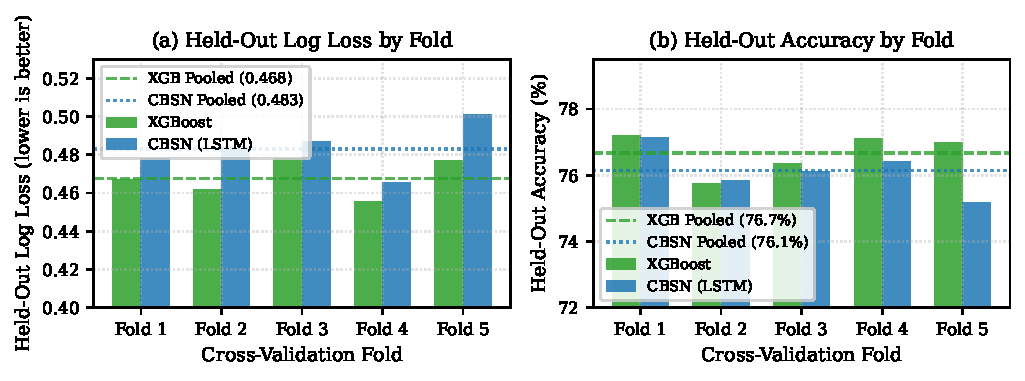
\includegraphics[width=0.92\textwidth]{fig2_heldout_metrics.pdf}
\caption{Held-out predictive performance across five bout-grouped cross-validation folds. (a) Held-out binary log loss (primary metric, lower is better): XGBoost consistently outperforms CBSN across all five test folds, achieving a pooled loss of 0.468 vs.\ 0.483. (b) Held-out classification accuracy (secondary metric, higher is better): XGBoost achieves 76.7\% pooled accuracy compared to 76.1\% for CBSN.}
\label{fig:cv_metrics}
\end{figure*}

As illustrated in Fig.~\ref{fig:cv_metrics}, XGBoost achieves a lower held-out log loss than CBSN on every single test fold. In the pooled evaluation ($N = 13,776$), XGBoost attains a log loss of 0.468 and an accuracy of 76.7\%, compared to 0.483 and 76.1\% for CBSN. 

In-sample, CBSN fits the training data well (accuracy 81.9\%, log-likelihood $-5355.27$), but falls short of the econometric model $M_2$ (accuracy 83.3\%, log-likelihood $-4817.02$, $\text{AIC} = 11,846$ vs.\ $17,139$).

\subsection{Attention Gate Dynamics and Memory Ablation}
Analyzing the CBSN attention gate weights reveals how the model balances immediate performance versus accumulated bout context across rounds (Fig.~\ref{fig:attention}). In early rounds (rounds 2--3), the mean historical weight $w_{\text{hist}}$ is $0.4178 \pm 0.003$ ($n = 3,777$). In championship rounds (rounds 11--12), $w_{\text{hist}}$ declines to $0.3074 \pm 0.005$ ($n = 984$). A paired within-bout comparison across 179 bouts completing 12 rounds confirms a statistically significant drop of $\Delta w_{\text{hist}} = -0.0637$ ($t = -3.40, p = 0.000845$). This neural attention decay aligns perfectly with our econometric finding in Model $M_2$: judges rely less on prior scorecard history as the final bell approaches.

To quantify whether the LSTM state $h_{r-1}$ actively generates catch-up predictions, we perform a counterfactual memory ablation on all test-fold rounds where a trailing corner was correctly predicted ($n = 1,476$). Holding round-$r$ punch metrics identical, we set $h_{r-1} = \mathbf{0}$. Erasing recurrent memory reduces the trailing corner's win probability by an average of $\Delta p = 0.0730 \pm 0.0061$ ($95\%\text{ CI: } [0.0669, 0.0791]$, $t = 23.44, p = 1.42 \times 10^{-103}$). This confirms that the recurrent state actively encodes compensatory bias.

\section{Discussion}

\subsection{Behavioral Mechanisms of Compensatory Officiating}
Our findings provide quantitative evidence that professional boxing judges exhibit significant sequential scorecard bias. Rather than treating rounds as independent 180-second contests, judges subconsciously award close rounds to trailing fighters. This behavior is consistent with cognitive theories of equity restoration and loss aversion~\cite{chen2016,peters2014}: when an arbiter perceives a contest becoming lopsided, ambiguous exchanges are resolved in favor of the trailing athlete to restore competitive balance.

The refutation of $H_2$ (weakened bias in rounds 11--12) provides crucial insight into referee psychology under extreme pressure. In early and middle rounds, judges may assume that ample time remains for the true victor to separate themselves, lowering the perceived cost of awarding a compensatory round. In championship rounds, however, the imminent finality of the official verdict, heightened public scrutiny, and athlete exhaustion make judges significantly more conservative, forcing greater adherence to raw punch volume and clean connections.

\subsection{Why Causal LSTMs Do Not Outperform Tree Ensembles}
Despite the conceptual elegance of modeling bout history via recurrent hidden states, our held-out cross-validation results show that XGBoost outperforms CBSN on both log loss (0.468 vs.\ 0.483) and accuracy (76.7\% vs.\ 76.1\%). Three architectural and domain factors explain this outcome:
\begin{enumerate}
    \item \textbf{Short Sequence Horizon:} Professional boxing matches span at most 12 rounds (mean sequence length in our dataset is $\sim 6.7$ rounds). For such short timelines, the cumulative scalar margin $\Delta_{ij,r-1}$ acts as an almost sufficient statistic for sequential history, leaving little residual signal for a 16-dimensional hidden state.
    \item \textbf{Tabular Sparsity and Observation Noise:} Biomechanical punch statistics exhibit high round-to-round variance. Gradient boosted decision trees excel at isolating step-function thresholds across tabular features, whereas recurrent neural networks are prone to fitting high-frequency noise.
    \item \textbf{Inductive Bias:} With 3,214 parameters, the CBSN exhibits slight out-of-sample over-smoothing, whereas XGBoost's constrained tree depth ($d=4$) enforces strict regularization.
\end{enumerate}

\subsection{Threats to Validity and Limitations}
Several limitations should be noted:
\begin{itemize}
    \item \textbf{Estimated Punch Proxies:} The objective baseline $\hat{P}$ is estimated from computer-vision tracking rather than ground-truth biomechanics. While DeepStrike demonstrates state-of-the-art accuracy~\cite{jabbr2023}, tracking artifacts may introduce measurement error.
    \item \textbf{Exclusion of Non-Standard Rounds:} Our panel focuses on 10--9 rounds, excluding rare 10--8 knockdown rounds and point deductions.
    \item \textbf{In-Sample Fixed Effects:} The high explanatory accuracy of $M_2$ (83.3\%) relies on bout fixed effects $\alpha_i$, which capture unobservable stylistic dynamics that cannot be computed prior to an unseen bout.
    \item \textbf{Absence of Open Scoring Control:} Under current ABC rules, scores remain hidden until the final decision. Evaluating whether compensatory bias vanishes under open scoring (as tested in certain regional jurisdictions) remains a compelling direction for future policy research.
\end{itemize}

\section{Conclusion}
This paper presents the first large-scale empirical evaluation of sequential bias and machine learning round prediction in professional boxing. Using 13,776 judge-rounds, we confirm that ringside judges exhibit pronounced compensatory catch-up bias ($H_1$: $\beta = -0.3016$), but show that this bias significantly attenuates during championship rounds ($H_2$ refuted, $\beta = +0.0990$). Furthermore, our supervised machine learning benchmark demonstrates that while sequential scorecard state provides predictive value, gradient boosted trees outperform causal deep sequence models on held-out bouts. These findings offer important empirical foundations for regulatory commissions considering automated AI judging aids and open scoring reforms. Code, trained-model summaries, and figure scripts are available at \repolink.

\bibliographystyle{IEEEtran}
\bibliography{references}

\end{document}
